\documentclass[tikz, margin=3mm, convert=pdf2svg]{standalone}
\usetikzlibrary{calc,arrows,automata,fit,backgrounds,shadows,positioning}
\usetikzlibrary{shapes.geometric,shapes.symbols}

\begin{document}

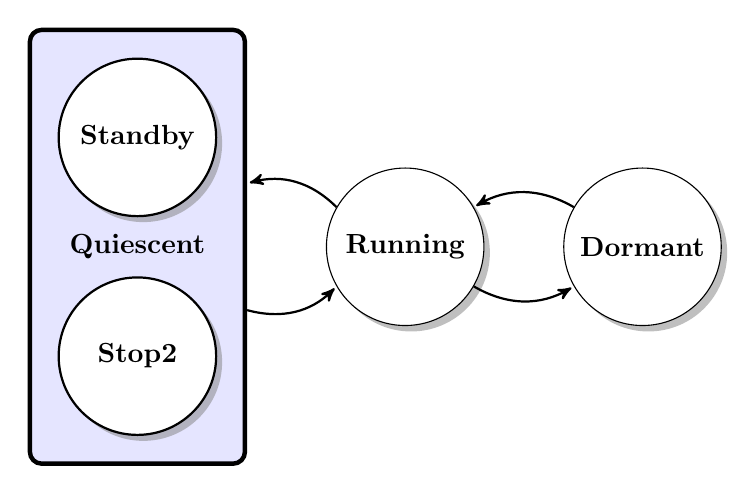
\begin{tikzpicture}[->,>=stealth',shorten >=1pt,auto,
  thick,state/.style={circle,draw,minimum size=2cm,fill=white,drop shadow, node distance = 1cm},
  state-group/.style = {rectangle,draw, fill=none, rounded corners=1.5mm,
                             inner ysep=2mm, inner xsep=4mm,
                             minimum height=6ex,
                             text width=18mm, align=center,node distance=2cm},
  every initial by arrow/.style={->>},
  initial text=init]
  \tikzstyle{surround} = [fill=blue!5,draw=black,rounded corners=2mm]

    \node[state] (SHUTDOWN) {\bf Standby};
    \node[state] (STOP) [below = 0.75cm of SHUTDOWN] {\bf Stop2};
    %\node[fill=none] (Label1) [below=of STOP, draw=none] {\bf Quiesent};
    \begin{pgfonlayer}{background}
    \node[state-group,inner sep=10pt] (Quiesent)
    [ fit = (SHUTDOWN) (STOP),fill=blue!10,ultra thick,label={center:{\bf Quiescent}}] {};
    \end{pgfonlayer}
    \node[state] (RUNNING) [right=of Quiesent] {\bf Running};
    \node[state] (DORMANT) [right=of RUNNING] {\bf Dormant};
    \path [thick] (RUNNING) edge [bend right] (DORMANT)
     (DORMANT) edge [bend right] (RUNNING)
     (RUNNING) edge [bend right] (Quiesent)
     (Quiesent) edge [bend right] (RUNNING);
  
  
  \end{tikzpicture}

  \end{document}